\documentclass[tikz,border=10pt]{standalone}
\usepackage{amsmath,amssymb}
\usetikzlibrary{arrows.meta,positioning,calc,decorations.pathmorphing}

\newcommand{\ord}{\operatorname{ord}}

\begin{document}
	
	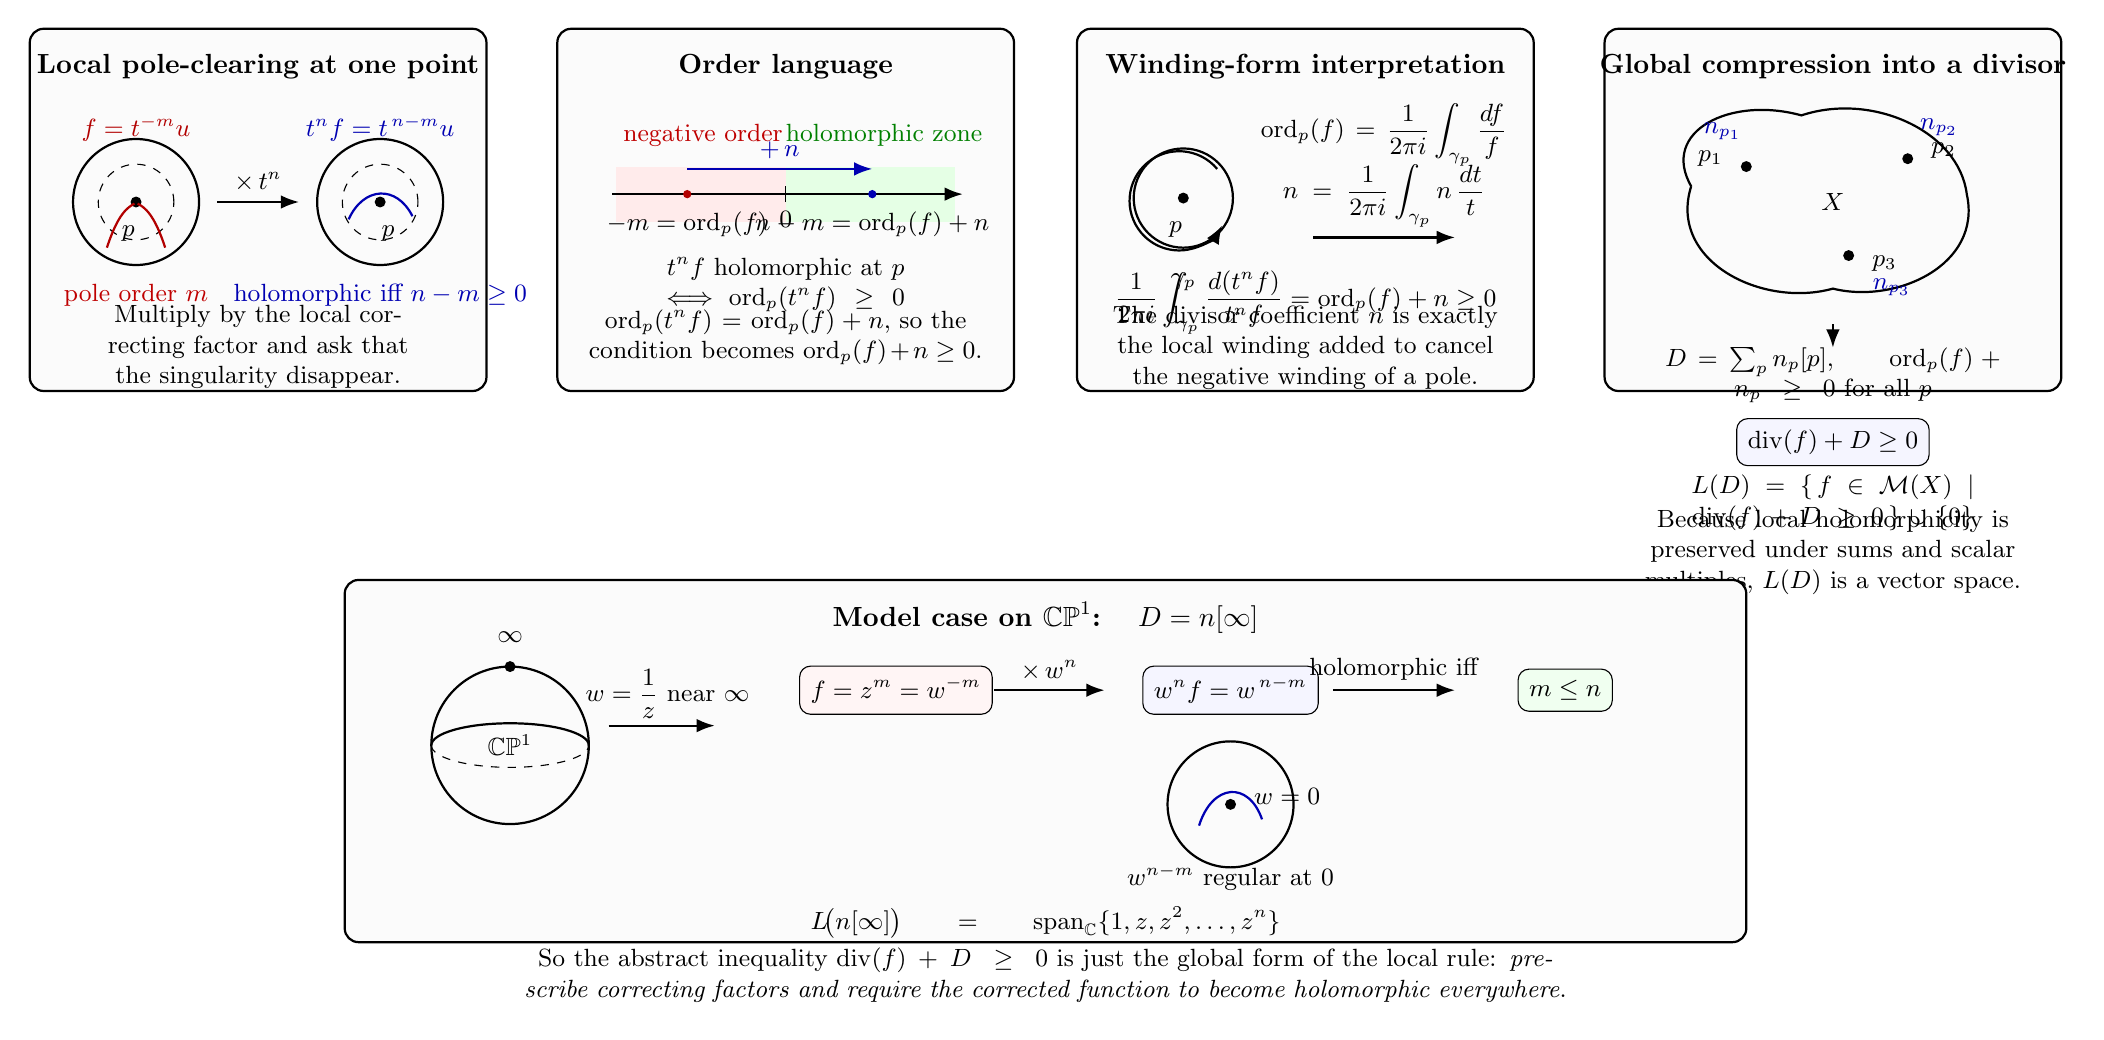
\begin{tikzpicture}[
		>=Latex,
		font=\small,
		panel/.style={draw, rounded corners=5pt, thick, fill=gray!3},
		title/.style={font=\bfseries},
		point/.style={circle, fill=black, inner sep=1.4pt},
		good/.style={blue!70!black, thick},
		bad/.style={red!70!black, thick},
		flow/.style={->, thick},
		every node/.style={align=center}
		]
		
		% =========================================================
		% PANEL A: local correction
		% =========================================================
		\begin{scope}[shift={(-10,3.3)}]
			\node[panel, minimum width=5.8cm, minimum height=4.6cm] (A) at (0,0) {};
			\node[title] at (0,1.82) {Local pole-clearing at one point};
			
			% left local disk
			\draw[thick] (-1.55,0.1) circle (0.8);
			\node[point,label={[xshift=-1mm,yshift=-1mm]below:$p$}] at (-1.55,0.1) {};
			\draw[dashed] (-1.55,0.1) circle (0.48);
			\node[bad] at (-1.55,1.03) {$f=t^{-m}u$};
			\node[red!75!black] at (-1.55,-1.08) {pole order $m$};
			
			% a little "blow-up" graphic
			\draw[bad] (-1.92,-0.48) .. controls (-1.78,-0.05) and (-1.66,0.03) .. (-1.57,0.08);
			\draw[bad] (-1.18,-0.48) .. controls (-1.32,-0.05) and (-1.44,0.03) .. (-1.53,0.08);
			
			% arrow
			\draw[flow] (-0.52,0.1) -- (0.52,0.1);
			\node[above] at (0,0.1) {$\times\, t^n$};
			
			% right local disk
			\draw[thick] (1.55,0.1) circle (0.8);
			\node[point,label={[xshift=1mm,yshift=-1mm]below:$p$}] at (1.55,0.1) {};
			\draw[dashed] (1.55,0.1) circle (0.48);
			\node[good] at (1.55,1.03) {$t^n f=t^{\,n-m}u$};
			\draw[good] (1.15,-0.12) .. controls (1.34,0.30) and (1.76,0.32) .. (1.96,-0.08);
			\node[blue!70!black] at (1.55,-1.08) {holomorphic iff $n-m\ge 0$};
			
			\node[text width=5.2cm] at (0,-1.74)
			{Multiply by the local correcting factor and ask that the singularity disappear.};
		\end{scope}
		
		% =========================================================
		% PANEL B: order shift
		% =========================================================
		\begin{scope}[shift={(-3.3,3.3)}]
			\node[panel, minimum width=5.8cm, minimum height=4.6cm] (B) at (0,0) {};
			\node[title] at (0,1.82) {Order language};
			
			% shaded regions
			\fill[red!8] (-2.15,-0.15) rectangle (0,0.55);
			\fill[green!10] (0,-0.15) rectangle (2.15,0.55);
			
			% axis
			\draw[thick,->] (-2.2,0.2) -- (2.25,0.2);
			\draw (0,0.1) -- (0,0.3);
			\node[below] at (0,0.1) {$0$};
			\node[below] at (-1.25,0.1) {$-m=\ord_p(f)$};
			\node[below] at (1.1,0.1) {$n-m=\ord_p(f)+n$};
			
			% points and arrow
			\fill[red!70!black] (-1.25,0.2) circle (1.5pt);
			\fill[blue!70!black] (1.1,0.2) circle (1.5pt);
			\draw[flow,blue!70!black] (-1.25,0.52) -- node[above] {$+\,n$} (1.1,0.52);
			
			\node[red!75!black] at (-1.05,0.95) {negative order};
			\node[green!50!black] at (1.25,0.95) {holomorphic zone};
			
			\node[text width=5.0cm] at (0,-0.95)
			{$t^n f$ holomorphic at $p$
				\;$\Longleftrightarrow$\;
				$\ord_p(t^n f)\ge 0$};
			
			\node[text width=5.0cm] at (0,-1.62)
			{$\ord_p(t^n f)=\ord_p(f)+n$,
				so the condition becomes
				$\ord_p(f)+n\ge 0$.};
		\end{scope}
		
		% =========================================================
		% PANEL C: winding picture
		% =========================================================
		\begin{scope}[shift={(3.3,3.3)}]
			\node[panel, minimum width=5.8cm, minimum height=4.6cm] (C) at (0,0) {};
			\node[title] at (0,1.82) {Winding-form interpretation};
			
			% loop and point
			\node[point,label={[xshift=-1mm,yshift=-1mm]below:$p$}] at (-1.55,0.15) {};
			\draw[thick] (-1.55,0.15) circle (0.63);
			\draw[->,thick] (-1.12,0.52) arc[start angle=40,end angle=330,radius=0.63];
			\node at (-1.55,-0.92) {$\gamma_p$};
			
			% formulas
			\node[text width=3.8cm] at (1.0,0.95)
			{$\displaystyle \ord_p(f)=\frac{1}{2\pi i}\int_{\gamma_p}\frac{df}{f}$};
			
			\node[text width=3.8cm] at (1.0,0.18)
			{$\displaystyle n=\frac{1}{2\pi i}\int_{\gamma_p}n\,\frac{dt}{t}$};
			
			\draw[flow] (0.1,-0.35) -- (1.9,-0.35);
			
			\node[text width=4.9cm] at (0,-1.18)
			{$\displaystyle \frac{1}{2\pi i}\int_{\gamma_p}\frac{d(t^n f)}{t^n f}
				=\ord_p(f)+n\ge 0$};
			
			\node[text width=5.1cm] at (0,-1.75)
			{The divisor coefficient $n$ is exactly the local winding added to cancel the negative winding of a pole.};
		\end{scope}
		
		% =========================================================
		% PANEL D: global divisor condition
		% =========================================================
		\begin{scope}[shift={(10,3.3)}]
			\node[panel, minimum width=5.8cm, minimum height=4.6cm] (D) at (0,0) {};
			\node[title] at (0,1.82) {Global compression into a divisor};
			
			% compact surface blob
			\draw[thick]
			(-1.8,0.3) .. controls (-2.2,1.0) and (-1.3,1.45) .. (-0.4,1.2)
			.. controls (0.5,1.5) and (1.6,1.0) .. (1.7,0.2)
			.. controls (1.9,-0.7) and (0.8,-1.2) .. (0,-1.0)
			.. controls (-0.9,-1.25) and (-2.1,-0.65) .. (-1.8,0.3);
			
			\node at (0,0.1) {$X$};
			
			% marked points
			\node[point,label={[xshift=-1mm,yshift=1mm]left:$p_1$}] at (-1.1,0.55) {};
			\node[point,label={[xshift=1mm,yshift=1mm]right:$p_2$}] at (0.95,0.65) {};
			\node[point,label={[xshift=1mm,yshift=-1mm]right:$p_3$}] at (0.2,-0.58) {};
			
			\node[blue!70!black] at (-1.4,1.0) {$n_{p_1}$};
			\node[blue!70!black] at (1.35,1.05) {$n_{p_2}$};
			\node[blue!70!black] at (0.75,-0.98) {$n_{p_3}$};
			
			\draw[flow] (0,-1.45) -- (0,-1.75);
			
			\node[text width=5.0cm] at (0,-2.1)
			{$D=\sum_p n_p[p],\qquad \ord_p(f)+n_p\ge 0\ \text{for all }p$};
			
			\node[draw, rounded corners=4pt, fill=blue!4, inner sep=4pt] at (0,-2.95)
			{$\operatorname{div}(f)+D\ge 0$};
			
			\node[text width=5.0cm] at (0,-3.72)
			{$\displaystyle L(D)=\{\,f\in\mathcal{M}(X)\mid \operatorname{div}(f)+D\ge 0\,\}\cup\{0\}$};
			
			\node[text width=5.0cm] at (0,-4.35)
			{Because local holomorphicity is preserved under sums and scalar multiples, $L(D)$ is a vector space.};
		\end{scope}
		
		% =========================================================
		% PANEL E: CP^1 model
		% =========================================================
		\begin{scope}[shift={(0,-3.7)}]
			\node[panel, minimum width=17.8cm, minimum height=4.6cm] (E) at (0,0) {};
			\node[title] at (0,1.82) {Model case on $\mathbb{CP}^1$: \; $D=n[\infty]$};
			
			% sphere / projective line
			\draw[thick] (-6.8,0.2) circle (1.0);
			\draw[dashed] (-7.8,0.2) arc[start angle=180,end angle=360,x radius=1.0,y radius=0.28];
			\draw[thick] (-5.8,0.2) arc[start angle=0,end angle=180,x radius=1.0,y radius=0.28];
			\node at (-6.8,0.2) {$\mathbb{CP}^1$};
			\node[point,label={[yshift=1mm]above:$\infty$}] at (-6.8,1.2) {};
			
			\node at (-4.8,0.85) {$w=\dfrac{1}{z}$ near $\infty$};
			\draw[flow] (-5.55,0.45) -- (-4.2,0.45);
			
			% monomial transformation
			\node[draw, rounded corners=4pt, fill=red!4, inner sep=4pt] at (-1.9,0.9)
			{$f=z^m=w^{-m}$};
			
			\draw[flow] (-0.65,0.9) -- (0.75,0.9);
			\node[above] at (0.05,0.9) {$\times\, w^n$};
			
			\node[draw, rounded corners=4pt, fill=blue!4, inner sep=4pt] at (2.35,0.9)
			{$w^n f=w^{\,n-m}$};
			
			\draw[flow] (3.65,0.9) -- (5.2,0.9);
			\node[above] at (4.42,0.9) {holomorphic iff};
			
			\node[draw, rounded corners=4pt, fill=green!6, inner sep=4pt] at (6.6,0.9)
			{$m\le n$};
			
			% local disk at infinity
			\draw[thick] (2.35,-0.55) circle (0.8);
			\node[point,label={[xshift=1mm,yshift=1mm]right:$w=0$}] at (2.35,-0.55) {};
			\draw[good] (1.95,-0.82) .. controls (2.12,-0.28) and (2.58,-0.25) .. (2.75,-0.74);
			\node at (2.35,-1.48) {$w^{n-m}$ regular at $0$};
			
			\node[text width=14.8cm] at (0,-2.05)
			{$\displaystyle L\!\bigl(n[\infty]\bigr)=\operatorname{span}_{\mathbb{C}}\{1,z,z^2,\dots,z^n\}$};
			
			\node[text width=15.6cm] at (0,-2.72)
			{So the abstract inequality $\operatorname{div}(f)+D\ge 0$ is just the global form of the local rule:
				\emph{prescribe correcting factors and require the corrected function to become holomorphic everywhere}.};
		\end{scope}
		
	\end{tikzpicture}
	
\end{document}